\chapter{REVISÃO BIBLIOGRÁFICA}

Em um trabalho de conclusão de curso de computação, a revisão bibliográfica é composta pela Fundamentação Teórica (\ref{fundamentacao-teorica}), Método de Desenvolvimento (\ref{metodo-de-desenvolvimento}) e os trabalhos relacionados (\ref{trabalhos-relacionados}). Na fundamentação teórica é onde são expostos os principais fundamentos que serão utilizados ao longo do desenvolvimento do trabalho. No método de trabalho, são descritos os processos de modelagem e desenvolvimento do protótipo. Em computação, o trabalho de conclusão de curso deve conter de 3 a 5 trabalhos relacionados (estado da arte).

\section{Fundamentação Teórica}
\label{fundamentacao-teorica}
É possível realizar citações diretas utilizando a \emph{chave} presente na bibliografia (\emph{referencias.bib}), como por exemplo \cite{turing}. Ou você pode inserir citações:

\begin{quote}
    The process of preparing programs for a digital computer is especially attractive, not only because it can be economically and scientifically rewarding, but also because it can be an aesthetic experience much like composing poetry or music.
    
    \rightline{{\rm --- \cite[p. 7]{knuth}}} 
\end{quote}

Para escrever fórmulas matemáticas, letras gregas e demais símbolos \emph{inline}, basta utilizar o comando \emph{\$}, como por exemplo 
$ x = \frac{-b \pm \sqrt{b^2 - 4ac}}{2a} $. 
Também é possível escrever fórmulas matemáticas como 
\( a^2 + b^2 = c^2 \)
dentro do texto. Fórmulas maiores podem ser escritas da seguinte forma:

\begin{equation} \label{eq1}
    \begin{split}
    \Delta = b^2 - 4ac \\
     x = \frac{-b \pm \sqrt{\Delta}}{2a}
    \end{split}
\end{equation}

\section{Método de Desenvolvimento}
\label{metodo-de-desenvolvimento}

\begin{figure}[H]
  \centering
  \caption{Método de Desenvolvimento do Trabalho}
 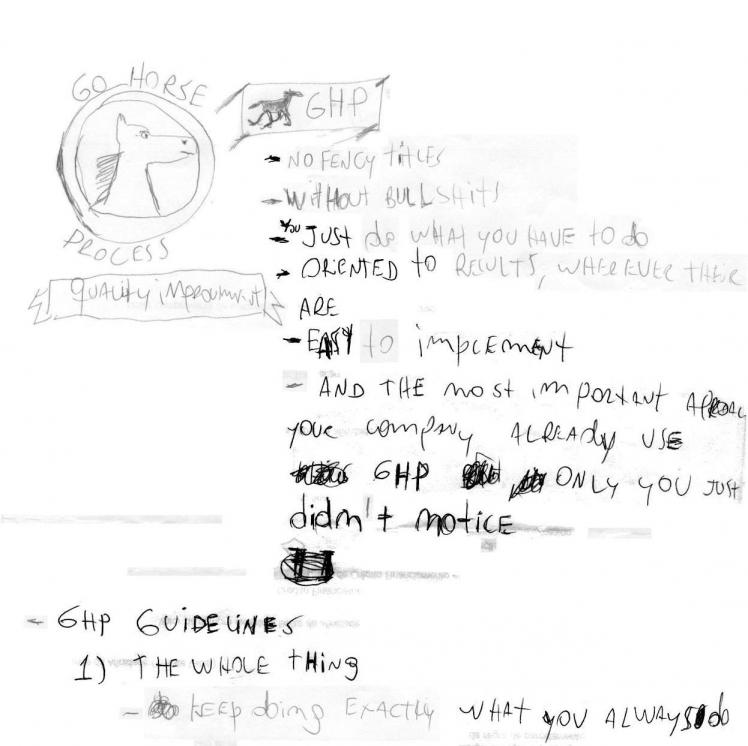
\includegraphics[scale=0.55]{imagens/gohorsenew.jpg} \par
\bigskip
\label{classes}
   Fonte: \cite{gohorse}
\end{figure}


\section{Trabalhos Relacionados}
\label{trabalhos-relacionados}
\subsection{Seção 1}

\subsubsection{Trabalho Relacionado 1}
\label{trab-relacionado-1}


\subsection{Trabalho Relacionado 2}
\label{tra-relacionado-2}


\subsection{Trabalho Relacionado 3}
\label{trab-relacionado-3}